% =====================================================================
% Undergraduate thesis (revised): Air Quality, Cost of Living, and Crime Across U.S. Counties
% Austin Yoo -- George Mason University, CDS 492
% Build: pdflatex capstone.tex (twice). Tables are read from ../output,
% figures from this folder; both are produced by ../analysis.R.
% =====================================================================
\documentclass[12pt,letterpaper]{report}

\usepackage[utf8]{inputenc}
\usepackage[T1]{fontenc}
\usepackage[margin=1in]{geometry}
\usepackage{setspace}
\usepackage{amsmath}
\usepackage{booktabs}
\usepackage{graphicx}
\usepackage{float}
\usepackage[font=small,labelfont=bf]{caption}
\usepackage{listings}
\usepackage{xcolor}
\usepackage[hidelinks]{hyperref}
\hypersetup{pdftitle={Air Quality, Cost of Living, and Crime Across U.S. Counties (Revised Edition)}, pdfauthor={Austin Yoo}}

\onehalfspacing

\lstset{
  language=R,
  basicstyle=\ttfamily\scriptsize,
  breaklines=true,
  numbers=left,
  numberstyle=\tiny,
  frame=single,
  showstringspaces=false,
  columns=fullflexible,
  keepspaces=true
}

\begin{document}

% ---------------------------------------------------------------------
% Front matter
% ---------------------------------------------------------------------
\pagenumbering{roman}

\begin{titlepage}
\centering
\vspace*{0.5in}
{\large\bfseries AIR QUALITY, COST OF LIVING, AND CRIME ACROSS U.S.\ COUNTIES}\\[1.5em]
by\\[0.5em]
Austin Yoo\\[1.5em]
An Undergraduate Thesis\\
Submitted to the\\
Faculty of the Department of Computational and Data Sciences\\
of\\
George Mason University\\
In Partial Fulfillment of\\
The Requirements for the Degree\\
of\\
Bachelor of Science\\
Computational and Data Sciences\\[2em]
\begin{flushleft}
\hspace{0.5in}Committee:\\[0.8em]
\hspace{0.5in}\rule{2.2in}{0.4pt}\hspace{0.2in}Dr.\ Kent Miller, Thesis Director\\[0.8em]
\end{flushleft}
\vspace{1em}
Date: Fall Semester 2025\\
Revised edition, October 2026\\[1.5em]
George Mason University\\
Fairfax, VA
\end{titlepage}

\thispagestyle{empty}
\begin{center}
{\bfseries Air Quality, Cost of Living, and Crime Across U.S.\ Counties}\\[1em]
An undergraduate thesis submitted in partial fulfillment of the requirements for the\\
degree of Bachelor of Science at George Mason University\\[1.5em]
by\\[0.5em]
Austin Yoo\\
Bachelor of Science, George Mason University, 2026\\[2em]
Director: Dr.\ Kent Miller, Professor\\
Department of Computational and Data Sciences\\[2em]
Fall Semester 2025\\
Revised edition, October 2026\\
George Mason University\\
Fairfax, VA
\end{center}
\clearpage

\thispagestyle{empty}
\vspace*{\fill}
\begin{center}
Copyright \copyright\ 2025 by Austin Yoo\\
All Rights Reserved
\end{center}
\vspace*{\fill}
\clearpage

\chapter*{Dedication}
\addcontentsline{toc}{chapter}{Dedication}
I dedicate this work to my family, peers, and professors, whose unwavering support and
belief in me made this journey possible. To my parents, for their endless encouragement;
to my friends and professors for their support of my studies; and to my future self, who
dared to ask the difficult questions and find answers in the data.
\clearpage

\chapter*{Acknowledgments}
\addcontentsline{toc}{chapter}{Acknowledgments}
I would like to express my deepest gratitude to those who supported me throughout this
thesis.

First, I thank my advisor, Dr.\ Kent Miller, whose guidance, insight, and patience shaped
this research from topic inception to final deliverable. His critical feedback and
encouragement improved the direction of this work in meaningful ways.

I am grateful to the faculty and staff of the Computational and Data Sciences Department
at George Mason University for providing the resources, seminars, and collaborative
environment that made this project possible.

I also thank the compilers of the public quality-of-life dataset used in this study, and
the U.S.\ government agencies whose records it is built from.

Lastly, I thank my family for believing in me, for tolerating my long hours, and for
reminding me why this work matters.
\clearpage

\tableofcontents
\clearpage
\listoftables
\clearpage
\listoffigures
\clearpage

\chapter*{Abstract}
\addcontentsline{toc}{chapter}{Abstract}
\begin{center}
{\bfseries AIR QUALITY, COST OF LIVING, AND CRIME ACROSS U.S.\ COUNTIES}\\[0.5em]
Austin Yoo, BS\\
George Mason University, 2025\\
Thesis Director: Dr.\ Kent Miller
\end{center}

\noindent People often choose where to live based on crime, cost of living, and
environmental quality. This thesis asks which of these place characteristics go along
with higher crime across U.S.\ counties. I use a public quality-of-life dataset that
combines 2016 reported crime per 1,000 residents with air quality, drinking-water
violations, cost of living, median income, unemployment, and population for 2,892 counties
in 49 states and the District of Columbia. A first version of this project ran the regressions on 87,457 public-school
rows. Because every school in a county shares the county's crime rate, and every county in a
state shares the state's air-quality value, those rows are not independent, and the
conventional standard error of the air-quality slope was about 15 times too small. I
therefore re-estimate the models at the county level with standard errors clustered by
state, add controls for population size, urbanization, income, and unemployment, and check
the results at the state level.

Three findings stand out. First, cost of living has no association with crime on its own
(slope $-0.33$ crimes per 1,000 per \$10{,}000, $p=0.62$); the significant result in the
first version came from the inflated sample. Second, better air quality goes with less
crime at first, but the association does not hold up: it halves once the controls are added
(one standard deviation of air quality goes with about one fewer crime per 1,000, or 5\% of
the mean, $p=0.03$), and it falls by another 60\% and is no longer significant ($p=0.36$)
when counties are compared only with others in the same Census region. Air quality mostly
stands in for broad geography, such as the dry, sunny West. Third, the features most strongly
associated with crime are median income (negative) and population size and urbanization
(positive). Unemployment and drinking-water violations show no association. The data are
cross-sectional, and crime is measured in 2016 while income and population are measured in
2022, so all results are associations, not causal effects.
\clearpage

\pagenumbering{arabic}

% ---------------------------------------------------------------------
% Chapter 1
% ---------------------------------------------------------------------
\chapter{Introduction}

Crime is not spread evenly across cities and regions. Researchers have offered many
explanations for why some places have more of it than others, including economic
disadvantage, weak institutions, social norms, and the built environment. More recently,
air and water pollution have been added to the list next to population density and
neighborhood structure. Pollution may affect crime directly, through its effects on the
brain, and indirectly, through stress, disorder, and weaker ties between neighbors
\cite{glaeser1999,sampson1997,bondy2020,reyes2007,hanna2016}.

\section{Research Questions}
This project was motivated by a practical question. People who move often compare places
by crime rate, cost of living, and environmental quality. If some of these features are
closely tied to crime, and if they can be changed by policy, it may be possible to lower
crime without asking people to move. I ask three questions:
\begin{enumerate}
\item Is air quality associated with county crime rates?
\item Is cost of living associated with county crime rates?
\item Among the features available in the data, which are most strongly associated with
crime once they are considered together?
\end{enumerate}

\section{Contribution and Scope}
A first version of this project answered the first two questions with simple regressions on
school-level records and found ``highly significant'' results for both. Working through the
structure of the data showed that those tests were not valid: the school rows repeat the same
county and state values many times. This revised version moves the analysis to the county
level, where crime is measured, uses standard errors clustered by state, and adds controls.
The revision changes the conclusions, and Chapter~\ref{ch:results} reports both the
original and the corrected estimates so the difference is clear. The analysis is
descriptive. It does not identify causal effects.

This edition, completed in October 2026, replaces the version submitted in December 2025
for the CDS 492 senior capstone course under the title ``The Impact of Social and Economic Factors on Increasing Crime.''

% ---------------------------------------------------------------------
% Chapter 2
% ---------------------------------------------------------------------
\chapter{Prior Research}

\section{Conceptual Framework}
Dense areas put potential offenders closer to potential victims. From a rational-choice
view, this lowers the cost of finding a target and raises the expected payoff of a crime.
Density also changes how neighbors interact. Depending on how close a neighborhood is and how
strong its institutions are, density can make informal social control stronger or weaker
\cite{glaeser1999,sampson1997}.

Air and water pollution are a separate group of factors. Exposure may affect behavior
through inflammation and reduced executive function \cite{bondy2020,reyes2007}. Some effects
are short-run, such as more people and targets in a dense area. Others are long-run, such as
childhood lead exposure. Community-level factors like collective efficacy sit between these
two and can shape both.

\section{Population Density and Crime Scaling}
Large cities have higher crime rates than small towns and rural areas. Glaeser and Sacerdote
\cite{glaeser1999} used victimization surveys, Uniform Crime Reports, and longitudinal data
to argue that density raises the returns to crime. Urban scaling research finds that many
social outcomes, including violent crime, grow faster than city population
\cite{bettencourt2007,bettencourt2013,oliveira2017}. These scaling laws describe averages
and do not predict any single city. At a finer scale, crime is concentrated in a small
share of places even inside dense cities \cite{weisburd2015}, so density alone does not
explain crime rates. Homicide rates also differ a lot between countries with similar levels
of urbanization, which points to governance and inequality as additional factors
\cite{unodc2023}.

\section{Collective Efficacy and Social Organization}
Sampson, Raudenbush, and Earls \cite{sampson1997} defined collective efficacy as mutual trust
among neighbors plus a shared willingness to step in when something goes wrong. In their
study of Chicago neighborhoods, higher collective efficacy went with lower violent crime,
even after accounting for the neighborhood's structural characteristics. Neighborhood
associations, religious groups, and community organizations can keep this kind of watchfulness
going. When ties between neighbors are weak, high density can instead increase anonymity.
Pollution and visible disorder may lower residents' willingness to act, so environmental
quality and social organization can feed into each other \cite{skogan1990}.

\section{Environmental Stress, Heat, and Aggression}
Heat has been linked to aggression in experiments and in field data \cite{anderson2000}.
Studies using administrative records find more violent crime and conflict when temperatures
are higher, after adjusting for seasonal patterns \cite{ranson2014,hsiang2013,burke2015}.
These studies fit the broader idea that environmental stress, from climate or from
pollution, can change behavior.

\section{Air Pollution and Violent Crime}
Bondy, Roth, and Sager \cite{bondy2020} used short-run changes in pollution and found that
crime rises when air pollution rises, even after controlling for weather and time. A separate
line of work shows that air pollution hurts cognitive performance \cite{chang2019}. That is
consistent with a biological explanation, although the evidence about crime itself is thinner
than the evidence about cognition.

\section{Lead, Water Pollution, and Developmental Effects}
Children exposed to lead show weaker impulse control and cognitive function. Reyes
\cite{reyes2007} used the phase-out of leaded gasoline and differences in exposure across
birth cohorts, and linked lower childhood lead exposure to less violent crime later. The
Flint, Michigan water crisis showed how failing infrastructure can raise blood lead levels
in children in vulnerable communities \cite{hanna2016,zahran2017}.

\section{Land Use, Guardianship, and Policing}
Routine activity theory says a crime happens when a motivated offender, a suitable target,
and the lack of a capable guardian come together \cite{cohen1979}. Land use touches all
three. Areas that mix housing and commercial space can have more targets and more anonymity,
while active businesses, residents, and community groups add guardianship. Hot-spot policing
focuses on the places where crime clusters \cite{braga2010}, and adding vegetation has been
associated with less crime in inner-city neighborhoods \cite{kuo2001}.

\section{Socioeconomic Inequality and Cumulative Environmental Risk}
Inequality affects both who is exposed to environmental hazards and who is at risk of crime
\cite{sampson1995,messner1997,currie2011}. Disorder in a neighborhood can make residents feel
less attached to it and weaken informal control \cite{skogan1990}. The built environment is
also linked to mental health \cite{evans2003}. For these reasons, pollution and crime should
be looked at alongside broader disadvantage and not as separate problems.

\section{Measurement, Identification, and Inference}
Prior studies mostly use one of three designs: cross-sectional comparisons with many
controls, panel models that use changes within a place over time, and quasi-experiments that
rely on a policy change or an environmental shock \cite{glaeser1999,bondy2020,reyes2007}.
Each has problems, such as spillovers between areas, crime moving somewhere else, and
differences in how crime is reported.

A separate problem matters for this project. When a variable is measured for a large group
(such as a state) but the regression is run on many smaller units inside each group (such as
schools), the observations within a group share the same value and are not independent.
Conventional standard errors then treat repeated copies as new information and can be far
too small \cite{moulton1990}. The usual fix is to cluster the standard errors at the level of
the group \cite{cameron2015}. My study is a cross-sectional comparison with controls and
state-clustered standard errors. It can describe associations but not cause and effect.

% ---------------------------------------------------------------------
% Chapter 3
% ---------------------------------------------------------------------
\chapter{Data}\label{ch:data}

\section{Source}
The data come from a public quality-of-life dataset posted on Kaggle \cite{vaughan}, built
to help people
choose a place to live. Its compiler merged several U.S.\ government sources, and its source
file lists them: reported crimes in 2016 from the FBI Uniform Crime Reporting county file
\cite{icpsr37059}; 2022 county population estimates \cite{census2022}; 2022 county
unemployment from the USDA Economic Research Service \cite{ers2022}; family cost of living
and median income from the Economic Policy Institute Family Budget Calculator
\cite{epi2024}; the share of days with a ``good'' Air Quality Index from the EPA
\cite{epaaqi}; drinking-water violations from the EPA Safe Drinking Water Information System
\cite{sdwis}; the 2020 presidential popular-vote winner by state \cite{app2020}; and public
school records from the National Center for Education Statistics \cite{nces2022}. The cost
of living builds on an earlier Kaggle county dataset \cite{asaniczka}.

The dataset comes in two forms: a county file with one row per county (3,134 rows) and a
school file with one row per public school (88,111 rows). The school file repeats its
county's values on every school row.

\section{Level of Measurement}
Table~\ref{tab:levels} shows the level at which each variable actually varies. This is the
key fact for the analysis. Crime, income, cost of living, unemployment, and population vary
by county. Air quality and the vote winner vary only by state: the air-quality variable takes
exactly one value per state and 50 distinct values in total. Any regression on air quality
therefore has, in effect, about 50 independent observations of it, no matter how many rows
are used.

\begin{table}[H]
\centering
\caption{Variables and the level at which they vary.}
\label{tab:levels}
\small
\begin{tabular}{@{}llll@{}}
\toprule
Variable & Unit & Varies by & Year \\
\midrule
Reported crime & per 1,000 residents & County & 2016 \\
Air quality & \% of days with ``good'' AQI & State only & -- \\
Drinking-water violations & count & County & -- \\
Cost of living (family budget) & \$ per year & County & -- \\
Median household income & \$ per year & County & 2022 \\
Cost-to-income ratio & \% & County & -- \\
Unemployment rate & \% & County & 2022 \\
Population & persons & County & 2022 \\
Urban share of schools & share (0--1) & County (from school file) & 2021--22 \\
2020 popular-vote winner & D / R & State & 2020 \\
\bottomrule
\end{tabular}
\end{table}

\section{Construction of the Analysis Sample}
I use the county file as the main data. Crime is stored as text such as ``14/1000'', which I
convert to crimes per 1,000 residents. It is rounded to whole numbers. 120 counties, almost
all very small, report a crime rate of exactly zero. A full year with no reported crime is
more likely to mean that the county did not report to the FBI program than that no crime
occurred, so I treat these as missing and check the result with them included.

The dataset has no land area, so I cannot compute population density directly. I measure
urbanization in two ways instead: the log of county population, and the share of the
county's public schools that the NCES classifies as being in a city or suburb. The school
file has no Illinois schools, so Illinois counties have no urban share. They drop out of
the main sample, and I check the result without the urban-share control so that they can
be included.

After these steps the analysis sample has 2,892 counties in 49 states and the District of
Columbia (50 state-level clusters; DC is a single county). Table~\ref{tab:desc} describes it.

\begin{table}[H]
\centering
\caption{Descriptive statistics, analysis sample of counties.}
\label{tab:desc}
\small
\begin{tabular}{@{}lrrrrr@{}}
\toprule
Variable & N & Mean & SD & Min & Max \\
\midrule
Crime per 1,000 residents (2016) & 2,892 & 19.83 & 11.92 & 1.00 & 89.00 \\
Air quality (\% good days) & 2,892 & 84.56 & 6.56 & 68.34 & 99.35 \\
Cost of living (\$) & 2,892 & 70,869 & 10,500 & 54,431 & 167,022 \\
Median income (\$) & 2,892 & 68,448 & 16,942 & 27,327 & 177,662 \\
Cost-to-income ratio (\%) & 2,892 & 107.08 & 19.17 & 52.00 & 236.97 \\
Unemployment rate (\%) & 2,892 & 3.72 & 1.32 & 1.34 & 17.19 \\
Population (2022) & 2,892 & 109,254 & 331,278 & 358 & 9,721,138 \\
Urban share of schools & 2,892 & 0.18 & 0.32 & 0.00 & 1.00 \\
Drinking-water violations & 2,620 & 2.96 & 11.05 & 0.00 & 456.00 \\
\bottomrule
\end{tabular}

\end{table}

\section{Data Limitations}
The variables come from different years. Crime is from 2016, while population, income, and
unemployment are from 2022, so the explanatory variables are measured after the outcome
(see Section~\ref{sec:limits}). Air quality is a single state-level figure and cannot reflect
differences between counties in the same state. Reported crime depends on what agencies
report, and the crime measure is rounded to whole numbers per 1,000.

% ---------------------------------------------------------------------
% Chapter 4
% ---------------------------------------------------------------------
\chapter{Hypotheses and Methods}

\section{Hypotheses}
\paragraph{Hypothesis 1 (air quality).} $H_0$: air quality has no linear association with
the county crime rate. $H_1$: it does. The literature in Chapter~2 suggests that better air
quality should go with less crime.

\paragraph{Hypothesis 2 (cost of living).} $H_0$: cost of living has no linear association
with the county crime rate. $H_1$: it does.

\section{Models}
For county $c$ in state $s$, the main specification is
\begin{equation}
\text{Crime}_{cs} = \beta_0 + \beta_1\,\text{AirQuality}_{s} + \beta_2\,\text{CostOfLiving}_{cs}
 + \mathbf{X}_{cs}'\boldsymbol{\gamma} + \varepsilon_{cs},
\end{equation}
where $\mathbf{X}$ holds the controls: log population, the urban share of schools, the
unemployment rate, log median income, and the cost-to-income ratio. Because cost of living
and median income are strongly correlated ($r=0.72$), the full model uses the cost-to-income
ratio, which measures how expensive a county is relative to what its residents earn. I
estimate five models:
\begin{enumerate}
\item[(1)] air quality only;
\item[(2)] cost of living only;
\item[(3)] air quality and cost of living together;
\item[(4)] air quality with all controls;
\item[(5)] all controls plus state fixed effects.
\end{enumerate}
Model~(5) compares counties only with other counties in the same state. This removes
everything that differs between states, including reporting practices, but it also removes
air quality, which varies only by state. It also drops the District of Columbia and Utah,
each of which has only one county in the sample, because a state with one county gives no
within-state comparison. Model~(5) therefore answers the third research
question for the county-level variables.

All models are ordinary least squares with standard errors clustered by state, which allows
counties in the same state to share unobserved shocks and accounts for the state-level
air-quality measure. Because there are only 50 clusters, $p$-values use a
$t$-distribution with 49 degrees of freedom. I use $\alpha = 0.05$. To compare variables measured in different units,
I also report standardized coefficients: the change in crime, in standard deviations, for a
one-standard-deviation change in each variable.

Because air quality varies only between states, it may simply pick up broad regional
differences. As a direct check, I add fixed effects for the four Census regions
(Northeast, Midwest, South, West) and, more finely, the nine Census divisions. These compare
states with more and fewer good-air days within the same part of the country.

% ---------------------------------------------------------------------
% Chapter 5
% ---------------------------------------------------------------------
\chapter{Results}\label{ch:results}

\section{Why the First Version Overstated Significance}
Table~\ref{tab:inference} starts with the original regression of crime on air quality,
estimated on 87,457 school rows. The slope is the same in the first two lines; only the
standard error changes. Treating the school rows as independent gives a $t$-statistic of
$-67$. Clustering by state, which recognizes that air quality takes only one value per
state, makes the standard error 15 times larger and the $t$-statistic falls to $-4.5$. The
same slope estimated on counties, or on the 50 states directly, gives similar conclusions:
the bivariate association is negative and significant, but far less precise than the first
version reported. The original cost-of-living regression had the same problem, because it
averaged school rows within ZIP codes and so repeated each county's values across its ZIP
codes.

\begin{table}[H]
\centering
\caption{Air quality and crime: the same bivariate slope under different units and standard
errors. Slope is crimes per 1,000 residents per percentage point of good-air days.}
\label{tab:inference}
\small
\begin{tabular}{@{}lcccc@{}}
\toprule
Specification & Slope & SE & $t$ & $p$ \\
\midrule
School rows, conventional SE (original) & $-0.369$ & $0.0055$ & $-67.45$ & $<10^{-16}$ \\
School rows, SE clustered by state & $-0.369$ & $0.0824$ & $-4.48$ & $<0.001$ \\
Counties, SE clustered by state & $-0.303$ & $0.0848$ & $-3.57$ & $<0.001$ \\
States (n = 50), robust SE & $-0.493$ & $0.2023$ & $-2.44$ & $0.018$ \\
\bottomrule
\end{tabular}

\end{table}

\section{Main Estimates}
Table~\ref{tab:main} reports the county models.

\begin{table}[H]
\centering
\caption{County regressions of crime per 1,000 residents. Standard errors clustered by state
in parentheses. $^{*}p<0.1$, $^{**}p<0.05$, $^{***}p<0.01$. Model~(5) drops the District of Columbia and Utah, which have one county each in the sample.}
\label{tab:main}
\small
\begin{tabular}{@{}lccccc@{}}
\toprule
 & (1) & (2) & (3) & (4) & (5) \\
\midrule
Air quality (\% good days) & $-0.303^{***}$ &  & $-0.301^{***}$ & $-0.154^{**}$ &  \\
 & $(0.085)$ &  & $(0.089)$ & $(0.068)$ &  \\[2pt]
Cost of living (\$10k) &  & $-0.329$ & $-0.153$ &  &  \\
 &  & $(0.651)$ & $(0.560)$ &  &  \\[2pt]
log population &  &  &  & $3.086^{***}$ & $3.724^{***}$ \\
 &  &  &  & $(0.458)$ & $(0.635)$ \\[2pt]
Urban share of schools &  &  &  & $10.415^{***}$ & $9.867^{***}$ \\
 &  &  &  & $(1.881)$ & $(1.938)$ \\[2pt]
Unemployment rate (\%) &  &  &  & $-0.202$ & $0.590$ \\
 &  &  &  & $(0.473)$ & $(0.388)$ \\[2pt]
log median income &  &  &  & $-27.781^{***}$ & $-32.434^{***}$ \\
 &  &  &  & $(5.338)$ & $(4.025)$ \\[2pt]
Cost-to-income ratio (\%) &  &  &  & $-0.127^{***}$ & $-0.206^{***}$ \\
 &  &  &  & $(0.046)$ & $(0.041)$ \\[2pt]
\midrule
State fixed effects & No & No & No & No & Yes \\
Counties & 2,892 & 2,892 & 2,892 & 2,892 & 2,890 \\
States (clusters) & 50 & 50 & 50 & 50 & 48 \\
$R^2$ & 0.028 & 0.001 & 0.028 & 0.320 & 0.448 \\
\bottomrule
\end{tabular}

\end{table}

\paragraph{Air quality.} On its own (Model~1), each additional percentage point of
good-air days goes with 0.30 fewer crimes per 1,000 residents ($p<0.001$). One standard
deviation of air quality (6.6 points) therefore goes with about 2.0 fewer crimes per 1,000,
or 10\% of the mean of 19.8. Air quality alone explains only 2.8\% of the variation between
counties. Adding the controls (Model~4) cuts the coefficient in half, to $-0.15$
($p=0.028$). One standard deviation now goes with about 1.0 fewer crime per 1,000, or 5\% of
the mean. Figure~\ref{fig:state} shows the same relationship across the 50 states, the level
at which air quality is measured. Across states the bivariate slope is $-0.49$ ($p=0.018$),
but after controlling for state urbanization and income it is $-0.42$ with $p=0.11$.

\begin{figure}[H]
\centering
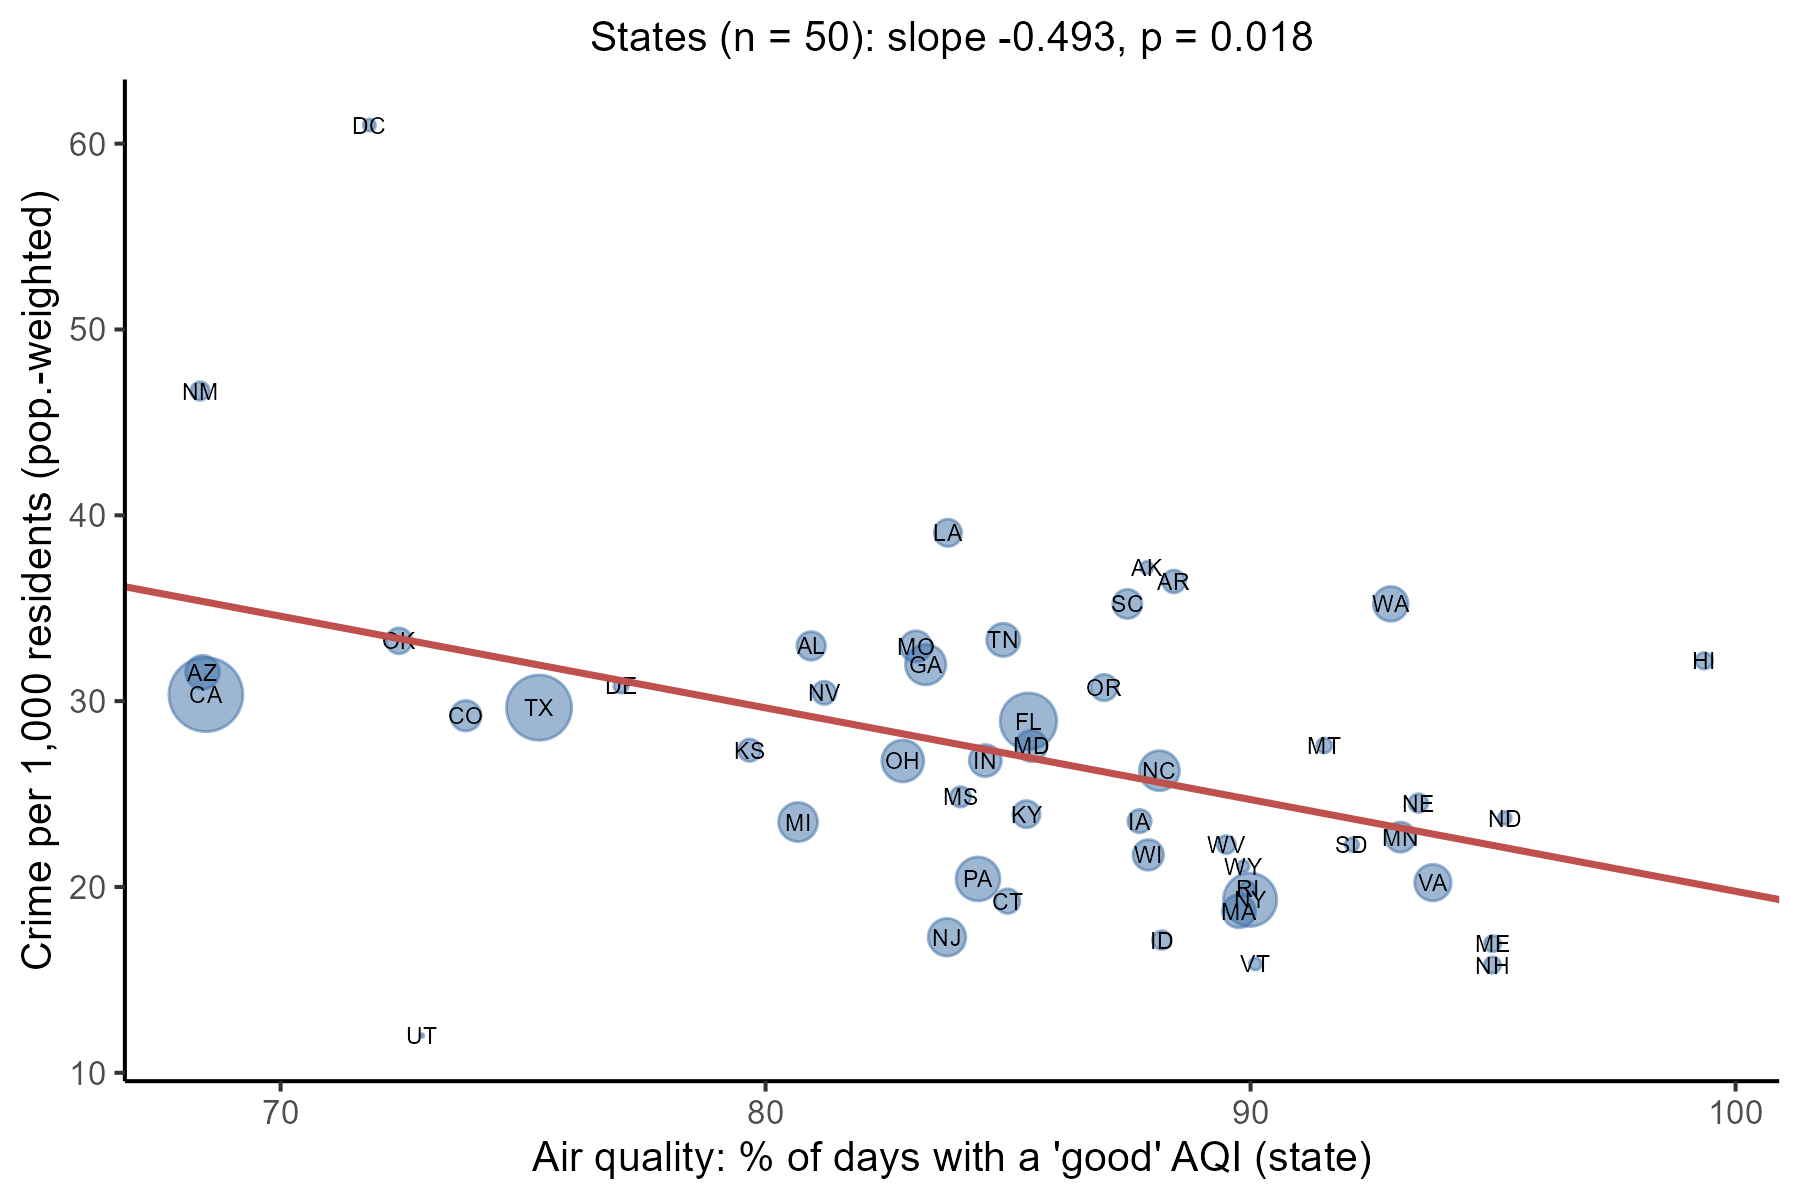
\includegraphics[width=0.88\textwidth]{fig_state_aqi.png}
\caption{Crime and air quality across states. Each point is a state; crime is the
population-weighted average over its counties, and point size reflects population. The line
is the OLS fit.}
\label{fig:state}
\end{figure}

\paragraph{Cost of living.} Cost of living has no association with crime on its own
(Model~2): the slope is $-0.33$ crimes per 1,000 per \$10{,}000, with a 95\% confidence
interval from $-1.64$ to $0.98$ and $p=0.62$. It also adds nothing when air quality is
included (Model~3). Figure~\ref{fig:col} shows why: across the range of cost of living, the
average crime rate is nearly flat. The reason becomes clear in Model~4. Expensive counties
tend to be both richer, which goes with less crime, and more urban, which goes with more
crime, and the two cancel out. Holding income and urbanization fixed, a county that is more
expensive relative to its income has somewhat less crime: a 10-point higher cost-to-income
ratio goes with 1.3 fewer crimes per 1,000 ($p=0.008$).

\begin{figure}[H]
\centering
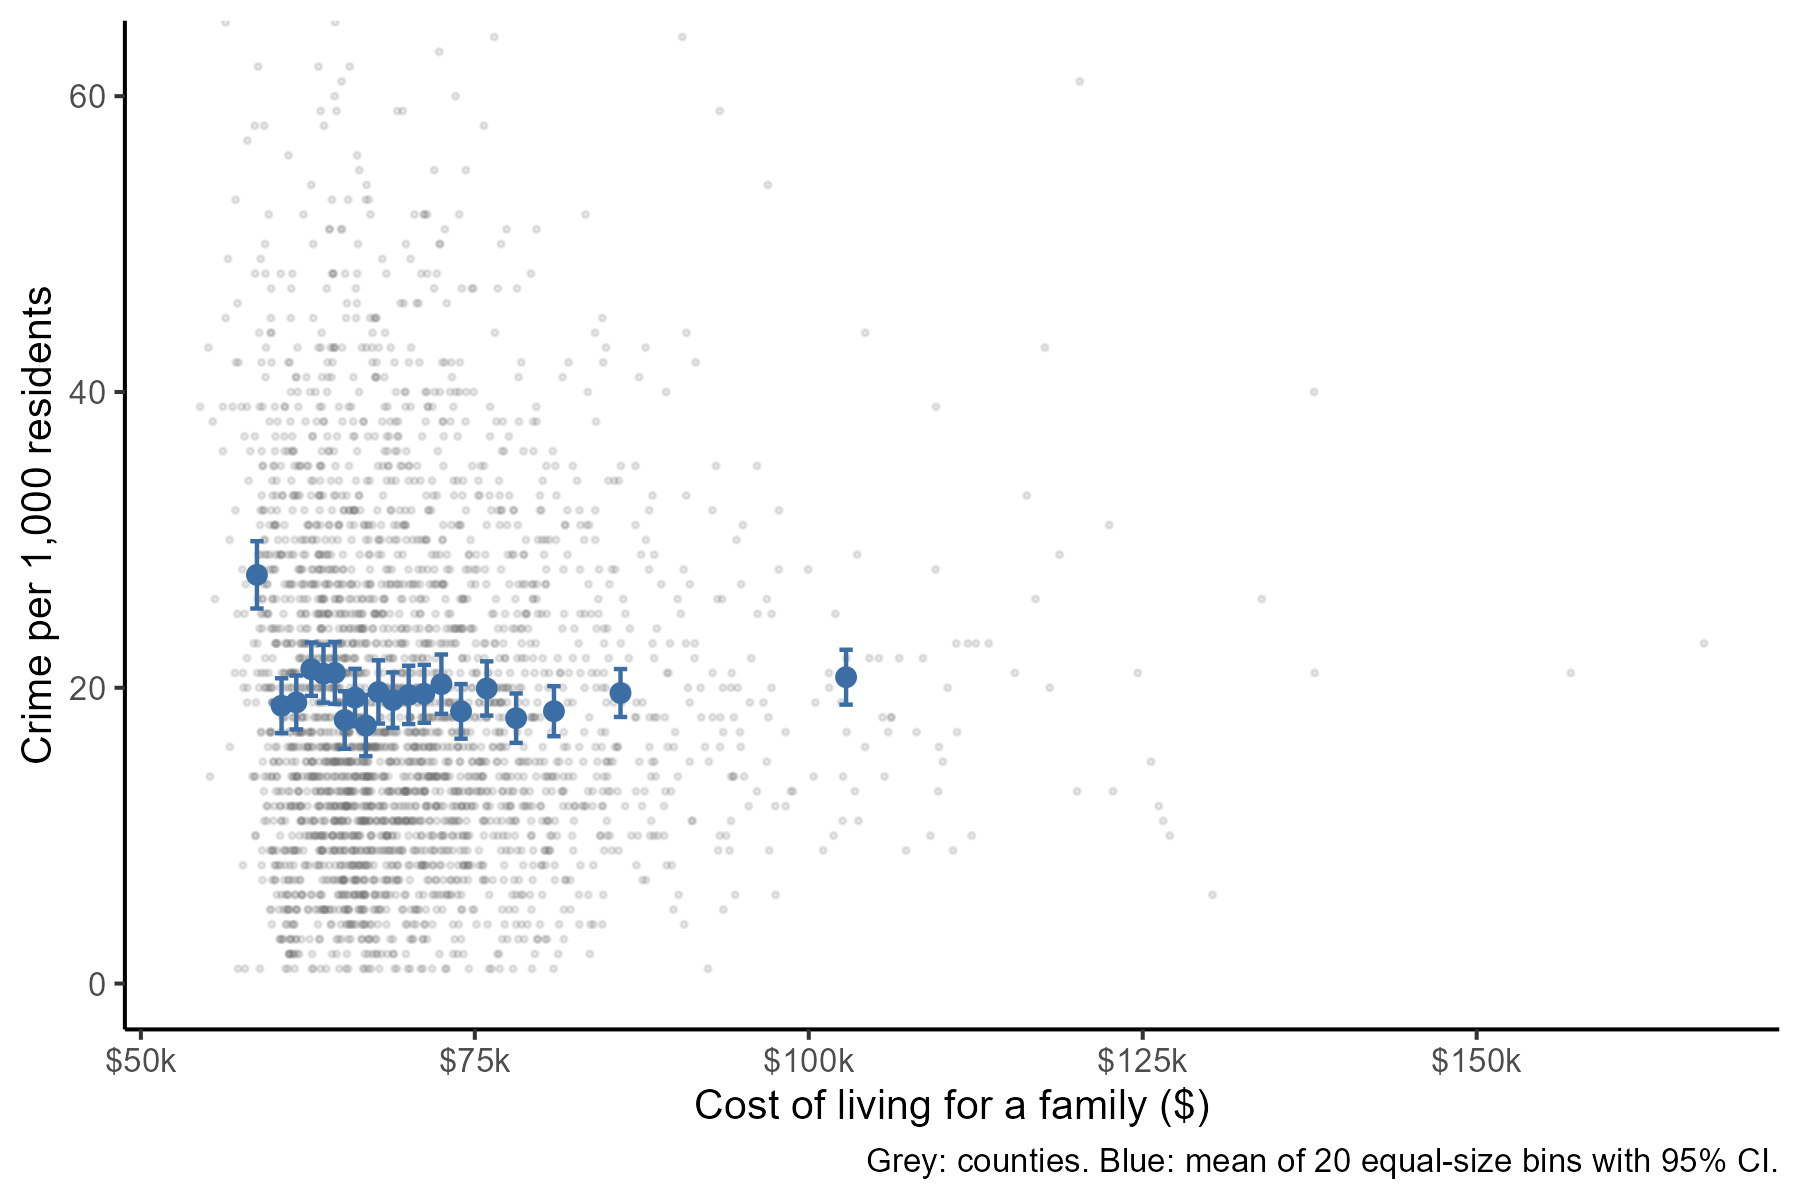
\includegraphics[width=0.88\textwidth]{fig_county_col.png}
\caption{Crime and cost of living across counties. Grey points are counties; blue points
are the mean crime rate in 20 equal-size groups of counties sorted by cost of living, with
95\% confidence intervals.}
\label{fig:col}
\end{figure}

\paragraph{Which features matter most.} Figure~\ref{fig:std} puts the variables on a common
scale. Median income has the strongest association: one standard deviation higher income
goes with 0.55 standard deviations less crime in Model~4 and 0.64 in Model~5. In crime
units, a county with 10\% higher median income has about 2.6 fewer crimes per 1,000. Next
come population size (0.38 to 0.46 SD) and the urban share of schools (0.26 to 0.28 SD),
both positive, and the cost-to-income ratio ($-0.20$ to $-0.33$ SD). Air quality is the
smallest of the significant variables ($-0.08$ SD). Unemployment shows no association in
either model. The controls raise the explained share of variation from 3\% to 32\%, and
state fixed effects raise it to 45\%.

\begin{figure}[H]
\centering
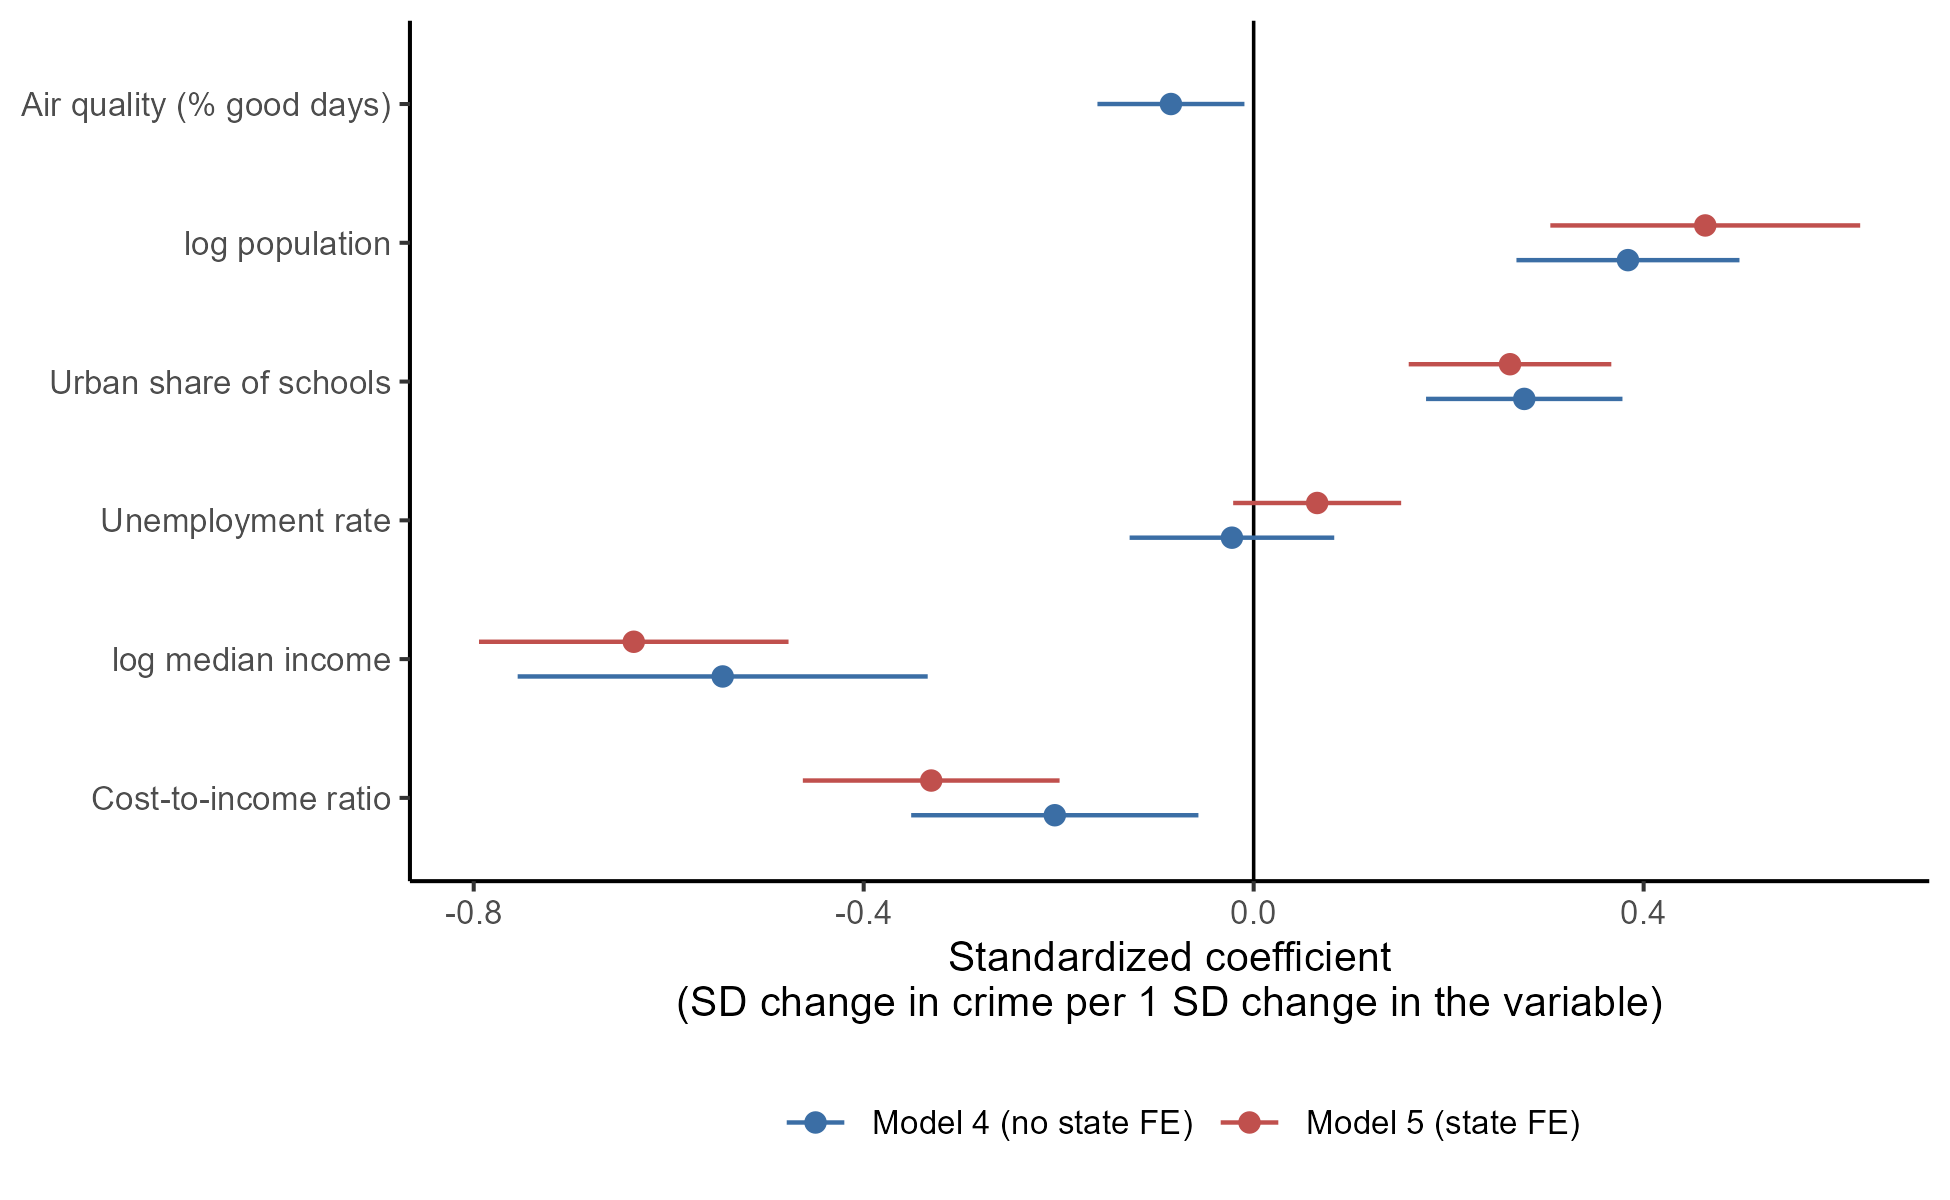
\includegraphics[width=0.92\textwidth]{fig_std_coefs.png}
\caption{Standardized coefficients with 95\% confidence intervals. Model~4 has no state fixed
effects; Model~5 compares counties within the same state, so air quality (a state-level
variable) drops out.}
\label{fig:std}
\end{figure}

\section{Robustness}
Table~\ref{tab:robust} changes one choice at a time in Model~4 and reports the air-quality
coefficient. Keeping the zero-crime counties, adding drinking-water violations, adding the
state vote winner, using cost of living instead of the cost-to-income ratio, or dropping the
urban-share control so that Illinois can be included all leave the coefficient between
$-0.14$ and $-0.19$ with $p$ between 0.020 and 0.047. Weighting counties by population,
which gives large urban counties more say, keeps a similar coefficient ($-0.19$) but the
standard error doubles and $p=0.19$. Drinking-water violations themselves show no
association with crime (coefficient $0.007$, $p=0.77$).

\paragraph{Air quality or geography?} The last two rows of Table~\ref{tab:robust} compare
counties only with other counties in the same Census region or division. With region fixed
effects the air-quality coefficient falls from $-0.15$ to $-0.06$ ($p=0.36$), and with
division fixed effects to $-0.05$ ($p=0.49$). This is not because the fixed effects remove
most of the variation in air quality: region explains only 13\% of the differences in air
quality between states, and the standard error barely changes (0.068 to 0.069). The
coefficient shrinks because the part of air quality that is related to crime is the part
shared within regions. Figure~\ref{fig:state} shows the pattern: the states with the fewest
good-air days are mostly in the West and Southwest (California, Arizona, New Mexico,
Colorado, Utah), where ozone and dust are common. The same check at the state level gives
the same answer ($-0.32$, $p=0.12$, $n=50$).

\begin{table}[H]
\centering
\caption{Robustness of the air-quality coefficient in Model~4. Standard errors clustered by
state.}
\label{tab:robust}
\small
\begin{tabular}{@{}lccc@{}}
\toprule
Variation of Model (4) & Air quality coef. (SE) & $p$ & Counties \\
\midrule
Keep counties reporting zero crime & $-0.165$ $(0.070)$ & $0.023$ & 3,004 \\
Weight counties by population & $-0.193$ $(0.144)$ & $0.188$ & 2,892 \\
Add drinking-water violations & $-0.156$ $(0.065)$ & $0.020$ & 2,620 \\
Add state 2020 vote winner (R = 1) & $-0.153$ $(0.074)$ & $0.043$ & 2,892 \\
Cost of living instead of cost-to-income & $-0.186$ $(0.077)$ & $0.020$ & 2,892 \\
Drop urban share (adds Illinois) & $-0.141$ $(0.069)$ & $0.047$ & 3,014 \\
Add Census region fixed effects (4) & $-0.063$ $(0.069)$ & $0.365$ & 2,892 \\
Add Census division fixed effects (9) & $-0.051$ $(0.072)$ & $0.488$ & 2,892 \\
\bottomrule
\end{tabular}

\end{table}

% ---------------------------------------------------------------------
% Chapter 6
% ---------------------------------------------------------------------
\chapter{Conclusion}

\section{Answers to the Research Questions}
\paragraph{Q1: Is air quality associated with crime?} Not in a reliable way. Counties in
states with more good-air days have lower crime, and the main county model rejects $H_0$ at
the 5\% level. But the association is much smaller than the first version suggested, and it
does not survive the checks. It halves once income and urbanization are taken into account,
loses significance when counties are weighted by population or when states are the unit, and
largely disappears when counties are compared within the same Census region or division.
The pattern is best read as a regional difference, with the West having both fewer good-air
days and somewhat higher crime, rather than as a link between air quality and crime. This
does not contradict the pollution literature in Chapter~2, which finds effects of
short-run changes in pollution on violent crime. A single state-level average of
good-air days is too coarse to detect such effects.

\paragraph{Q2: Is cost of living associated with crime?} No. I fail to reject $H_0$
($p=0.62$). The significant result in the first version was an artifact of repeating county
values across school and ZIP-code rows. Cost of living matters only in relation to income:
among counties with the same income and urbanization, those that are more expensive have
somewhat less crime.

\paragraph{Q3: Which features matter most?} Income and urbanization. Median income has the
strongest association (negative), followed by population size and the urban share of
schools (both positive). Air quality has the weakest association and is not robust to
regional comparisons, and unemployment and drinking-water violations show none. These results match the older
literature on density, opportunity, and disadvantage in Chapter~2 better than the newer
environmental literature.

\section{Lesson on Method}
The largest change between the two versions came from the unit of analysis, not from a new
model. A regression on 87,457 rows looked overwhelmingly significant, but the variable of
interest had only 50 distinct values. Matching the unit of analysis to the level at which the
data are measured, and clustering the standard errors at that level, is a basic step that
changes the conclusions here. A second lesson is that a variable measured for large areas can
easily stand in for geography. Comparing within regions is a simple way to check this.

\section{Limitations}\label{sec:limits}
\begin{itemize}
\item \textbf{Associations only.} The data are a single cross-section. Unmeasured
differences between places, such as policing, age structure, or poverty concentration,
could explain the associations.
\item \textbf{Coarse air-quality measure.} Air quality is one number per state, so the
analysis cannot use differences in pollution between counties, and it has effectively 50
observations.
\item \textbf{Reversed timing.} Crime is measured in 2016, but income, unemployment, and
population are measured in 2022, six years later. The explanatory variables therefore come
after the outcome they are meant to explain. This rules out reading them as causes of crime,
and if crime itself affects later income or population, for example by pushing residents
out, the associations could partly run in the opposite direction. The estimates assume that
the ranking of counties on these variables changed little between 2016 and 2022.
\item \textbf{Crime reporting.} The crime measure covers reported crimes only, is rounded to
whole numbers per 1,000, and treats zero-crime counties as non-reporting.
\item \textbf{No population density.} Without land area, urbanization is measured with
population size and school locale codes. Illinois has no school records and is missing from
the main sample.
\item \textbf{Regional data.} Relationships across counties do not describe the behavior of
individual people.
\end{itemize}

\section{Future Work}
The most useful next step is a county-level pollution measure, such as annual PM$_{2.5}$
from EPA monitors or satellite estimates, matched to crime in the same year. A panel of
counties over several years would allow comparisons within the same county over time, which
removes stable differences between places. Sudden pollution shocks, such as wildfire smoke,
would come closer to the causal designs reviewed in Chapter~2. Adding land area, poverty,
and age structure from the Census would also strengthen the county model.

% ---------------------------------------------------------------------
% Appendix
% ---------------------------------------------------------------------
\appendix
\chapter{Software}
The first version of this project was written in R with \texttt{ggplot2}, \texttt{dplyr},
and \texttt{janitor}. The revised analysis is also written in R (version 4.3.2), using \texttt{dplyr} and
\texttt{readr} for data preparation, \texttt{fixest} for the regressions and clustered
standard errors, \texttt{ggplot2} for the figures, and \texttt{jsonlite} to save the numbers
quoted in the text. It reads the county and school files,
builds the analysis sample, estimates all models, and writes every table and figure in this
document. The full script is below.

\lstinputlisting{../analysis.R}

% ---------------------------------------------------------------------
% Bibliography
% ---------------------------------------------------------------------
\begin{thebibliography}{99}
\addcontentsline{toc}{chapter}{Bibliography}

\bibitem{glaeser1999} Edward L. Glaeser and Bruce Sacerdote. Why is there more crime in
cities? \textit{Journal of Political Economy}, 107(S6):S225--S258, 1999.

\bibitem{sampson1997} Robert J. Sampson, Stephen W. Raudenbush, and Felton Earls.
Neighborhoods and violent crime: A multilevel study of collective efficacy.
\textit{Science}, 277(5328):918--924, 1997.

\bibitem{bondy2020} Malvina Bondy, Sefi Roth, and Lutz Sager. Crime is in the air: The
contemporaneous relationship between air pollution and crime. \textit{Journal of the
Association of Environmental and Resource Economists}, 7(3):555--585, 2020.

\bibitem{reyes2007} Jessica W. Reyes. Environmental policy as social policy? The impact of
childhood lead exposure on crime. \textit{The B.E. Journal of Economic Analysis \& Policy},
7(1), 2007.

\bibitem{hanna2016} Mona Hanna-Attisha, Jenny LaChance, Richard C. Sadler, and Allison
Champney Schnepp. Elevated blood lead levels in children associated with the Flint
drinking water crisis: A spatial analysis of risk and public health response.
\textit{American Journal of Public Health}, 106(2):283--290, 2016.

\bibitem{unodc2023} United Nations Office on Drugs and Crime. \textit{Global Study on
Homicide 2023}. United Nations, 2023.

\bibitem{bettencourt2007} Lu\'is M. A. Bettencourt, Jos\'e Lobo, Dirk Helbing, Christian
K\"uhnert, and Geoffrey B. West. Growth, innovation, scaling, and the pace of life in
cities. \textit{PNAS}, 104(17):7301--7306, 2007.

\bibitem{bettencourt2013} Lu\'is M. A. Bettencourt. The origins of scaling in cities.
\textit{Science}, 340(6139):1438--1441, 2013.

\bibitem{oliveira2017} Marcos Oliveira, Carmelo Bastos-Filho, and Ronaldo Menezes. The
scaling of crime concentration in cities. \textit{PLoS ONE}, 12(8):e0183110, 2017.

\bibitem{weisburd2015} David Weisburd. The law of crime concentration and the criminology
of place. \textit{Criminology}, 53(2):133--157, 2015.

\bibitem{cohen1979} Lawrence E. Cohen and Marcus Felson. Social change and crime rate
trends: A routine activity approach. \textit{American Sociological Review}, 44(4):588--608,
1979.

\bibitem{anderson2000} Craig A. Anderson. Temperature and aggression. \textit{Advances in
Experimental Social Psychology}, 32:63--133, 2000.

\bibitem{ranson2014} Matthew Ranson. Crime, weather, and climate change. \textit{Journal of
Environmental Economics and Management}, 67(3):274--302, 2014.

\bibitem{hsiang2013} Solomon M. Hsiang, Marshall Burke, and Edward Miguel. Quantifying the
influence of climate on human conflict. \textit{Science}, 341(6151):1235367, 2013.

\bibitem{burke2015} Marshall Burke, Solomon M. Hsiang, and Edward Miguel. Climate and
conflict. \textit{Annual Review of Economics}, 7:577--617, 2015.

\bibitem{chang2019} Tom Y. Chang, Joshua Graff Zivin, Tal Gross, and Matthew Neidell. The
effect of pollution on worker productivity: Evidence from call center workers in China.
\textit{American Economic Journal: Applied Economics}, 11(1):151--172, 2019.

\bibitem{currie2011} Janet Currie. Inequality at birth: Some causes and consequences.
\textit{American Economic Review}, 101(3):1--22, 2011.

\bibitem{zahran2017} Sammy Zahran, Shawn P. McElmurry, and Richard C. Sadler. Four phases
of the Flint water crisis: Evidence from blood lead levels in children.
\textit{Environmental Research}, 157:160--172, 2017.

\bibitem{braga2010} Anthony A. Braga and David L. Weisburd. \textit{Policing Problem Places:
Crime Hot Spots and Effective Prevention}. Oxford University Press, 2010.

\bibitem{kuo2001} Frances E. Kuo and William C. Sullivan. Environment and crime in the
inner city: Does vegetation reduce crime? \textit{Environment and Behavior},
33(3):343--367, 2001.

\bibitem{sampson1995} Robert J. Sampson and William Julius Wilson. Toward a theory of race,
crime, and urban inequality. In John Hagan and Ruth D. Peterson, editors, \textit{Crime and
Inequality}, pages 37--54. Stanford University Press, 1995.

\bibitem{messner1997} Steven F. Messner and Richard Rosenfeld. \textit{Crime and the
American Dream}. Wadsworth, 2nd edition, 1997.

\bibitem{skogan1990} Wesley G. Skogan. \textit{Disorder and Decline: Crime and the Spiral
of Decay in American Neighborhoods}. Free Press, 1990.

\bibitem{evans2003} Gary W. Evans. The built environment and mental health. \textit{Journal
of Urban Health}, 80(4):536--555, 2003.

\bibitem{moulton1990} Brent R. Moulton. An illustration of a pitfall in estimating the
effects of aggregate variables on micro units. \textit{Review of Economics and Statistics},
72(2):334--338, 1990.

\bibitem{cameron2015} A. Colin Cameron and Douglas L. Miller. A practitioner's guide to
cluster-robust inference. \textit{Journal of Human Resources}, 50(2):317--372, 2015.

\bibitem{icpsr37059} United States Department of Justice, Federal Bureau of Investigation.
\textit{Uniform Crime Reporting Program Data: County-Level Detailed Arrest and Offense Data,
United States, 2016}. ICPSR 37059, Inter-university Consortium for Political and Social
Research. \url{https://doi.org/10.3886/ICPSR37059.v3}.

\bibitem{census2022} U.S. Census Bureau. County population totals: 2020--2022 (Vintage
2022 population estimates).
\url{https://www.census.gov/data/datasets/time-series/demo/popest/2020s-counties-total.html}.

\bibitem{ers2022} U.S. Department of Agriculture, Economic Research Service. County-level
data sets: Unemployment and median household income.
\url{https://www.ers.usda.gov/data-products/county-level-data-sets/}.

\bibitem{epi2024} Economic Policy Institute. Family Budget Calculator.
\url{https://www.epi.org/resources/budget/}.

\bibitem{epaaqi} U.S. Environmental Protection Agency. Outdoor air quality data: Air
Quality Index report. \url{https://www.epa.gov/outdoor-air-quality-data}.

\bibitem{sdwis} U.S. Environmental Protection Agency. Safe Drinking Water Information
System (SDWIS) federal reports.
\url{https://ordspub.epa.gov/ords/sfdw_rest/r/sfdw/sdwis_fed_reports_public/}.

\bibitem{app2020} The American Presidency Project. 2020 presidential election statistics.
\url{https://www.presidency.ucsb.edu/statistics/elections/2020}.

\bibitem{nces2022} National Center for Education Statistics. Public school characteristics,
2021--22. \url{https://catalog.data.gov/dataset/public-school-characteristics-current-8d621}.

\bibitem{vaughan} Zac Vaughan. City/ZIP/County/FIPS -- Quality of Life (US). Kaggle.
\url{https://www.kaggle.com/datasets/zacvaughan/cityzipcountyfips-quality-of-life}.

\bibitem{asaniczka} asaniczka. US cost of living dataset (3171 counties). Kaggle.
\url{https://www.kaggle.com/datasets/asaniczka/us-cost-of-living-dataset-3171-counties}.

\end{thebibliography}

% ---------------------------------------------------------------------
% Biography
% ---------------------------------------------------------------------
\chapter*{Biography}
\addcontentsline{toc}{chapter}{Biography}
Austin Yoo is completing a Bachelor of Science in Computational and Data Sciences at
George Mason University, with a minor in Business and an expected graduation in May 2026.
He is interested in environmental data, social behavior, decision making, simulation
modeling, and machine learning applied to social and economic systems.

During his studies he worked on projects about crime prediction, housing market trends, and
social behavior simulations using Python, R, and NetLogo. His business minor coursework
covered business analytics, management, and IT strategy.

After graduation he plans to keep doing research on social, economic, and financial behavior
with data science, mainly analytical modeling and financial technology.

\end{document}
